\section{内核功能实现}\label{sec:KernelFunctionalityImplementation}

内核是操作系统的核心组件,负责管理内存和设备,同时为软件应用程序提供使用这些资源的接口。根据复杂性和目标的不同,内核的开发可以遵循不同的模型。主要有两种模型:微内核和宏内核。微内核的目标是将大多数服务运行在用户空间,从而提高安全性和模块化。

MinmusOS 采用的是宏内核模式,因此其所有服务和设备驱动程序都在单一地址空间内运行,并处于特权模式下。这种模式提高了效率并减少了代码复杂性,但缺点是其中任何一个组件的错误都可能导致整个系统崩溃。

在本节(\cref{sec:KernelFunctionalityImplementation})中,笔者将详细探讨 MinmusOS 内核各项功能的实现,包括中断管理、驱动程序、多任务处理、系统调用、命令行解释器、内存管理以及文件系统。

\subsection{中断(Interrupts)}

\subsubsection{中断描述符表(Interrupt Descriptor Table)}

\subsubsection{中断服务例程(Interrupt Service Routines)}

\subsubsection{CPU 异常(CPU Exceptions)}

\subsubsection{可编程中断控制器(Programmable Interrupt Controller)}

在代码中添加 \texttt{asm!("int \$0");} 可以触发除零中断,如\cref{fig:InterruptHandlerPresentation},MinmusOS 提供了友好的用户交互。蓝屏界面采用了经典的蓝底白字风格,类似于传统的Windows蓝屏死机(BSOD),并显示了详细的错误信息,包括错误类型和技术信息(如错误代码、指令指针、代码段、扩展标志等),有助于开发人员定位问题,便于调试和修复。

\begin{figure}[htbp]
    \centering
    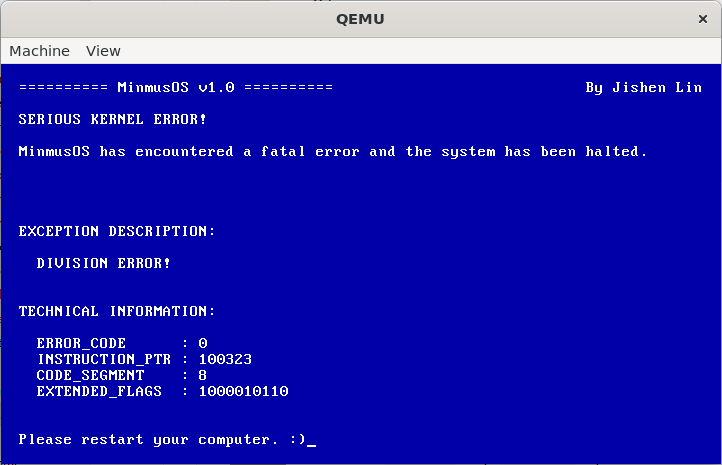
\includegraphics[width=0.8\textwidth]{figures/InterruptHandlerPresentation.png}
    \caption{中断处理器演示}
    \label{fig:InterruptHandlerPresentation}
\end{figure}

\subsection{驱动程序(Drivers)}

\subsubsection{键盘驱动程序(Keyboard Driver)}

\subsubsection{高级技术附件磁盘驱动程序(Advanced Technology Attachment Disk Driver)}

\subsection{多任务处理(Multitasking)}

\subsubsection{上下文切换(Context Switching)}

\subsubsection{CPU 调度器(CPU Scheduler)}

\subsubsection{任务管理器(Task Manager)}

\subsection{系统调用(System Calls)}

\subsection{命令行解释器(Shell)}

\subsection{内存管理(Memory Management)}

\subsection{文件系统(File System)}